% main.tex chỉ chứa \input; mỗi người sửa file riêng trong sections/.
% Biên dịch: pdflatex main && bibtex main && pdflatex main && pdflatex main (hoặc Overleaf, pdfLaTeX).
% Style: ACL (acl.sty). Đổi [review] <-> bỏ option để chuyển bản ẩn danh / bản cuối.
\documentclass[11pt]{article}
\usepackage[review]{acl}

\usepackage{times}
\usepackage{latexsym}
\usepackage[T5,T1]{fontenc}   % T5 cho tiếng Việt (chỉ dùng trong \vi{...}); T1 là mặc định
\usepackage[utf8]{inputenc}
\usepackage{lmodern}          % cung cấp font T5
\usepackage{microtype}
\usepackage{booktabs}
\usepackage{array}
\usepackage{graphicx}
\usepackage{amsmath}
\usepackage{tikz}
\usetikzlibrary{positioning,arrows.meta}

% Chữ tiếng Việt: luôn bọc trong \vi{...}
\newcommand{\vi}[1]{{\fontencoding{T5}\fontfamily{lmr}\selectfont #1}}
\newcommand{\texttvi}[1]{{\fontencoding{T5}\fontfamily{lmtt}\selectfont #1}}
% Đánh dấu chỗ cần đồng bộ với người khác (xoá trước khi nộp)
\newcommand{\todo}[1]{\textcolor{red}{[TODO: \vi{#1}]}}
\usepackage{xcolor}

\title{TODO Title: Structure-Aware Document-Level EN$\leftrightarrow$VI Legal Translation\\with a Fine-Tuned 1.8B Model}

% Tác giả (bản cuối). Ở chế độ [review], acl.sty tự ẩn.
\author{Pham Thi Khanh Linh \\ \texttt{TODO} \And
        Nguyen Thi Hien Trang \\ \texttt{TODO} \And
        TODO (L\^am) \\ \texttt{TODO}}

\begin{document}
\maketitle

% Người phụ trách: TRANG. Viết/chỉnh sau khi Linh xong Results (số liệu lấy từ đó).
% TODO(nhóm): chốt "claim" của bài (dàn ý yêu cầu). Câu dưới chỉ nêu điều có số liệu chống lưng.
\begin{abstract}
We describe our system for the VLSP 2026 shared task on English$\leftrightarrow$Vietnamese legal machine translation, where whole Markdown documents are translated by a model of fewer than 3B parameters that runs locally without external APIs, and inference time and memory are also evaluated.
We fine-tune Hy-MT2-1.8B with LoRA on segment-level legal data and run it inside a structure-aware document pipeline: Markdown is parsed into nodes, prose is packed into blocks without marker tokens, outputs are checked for lost headings, labels, uncovered source and unfinished generations, and failed units get one recovery pass with a changed input.
On the 50-document public test, an earlier version of the pipeline gains $+1.2$ (EN$\to$VI) and $+1.4$ (VI$\to$EN) BLEU by packing neighbouring nodes into one request instead of translating nodes one by one.
A second LoRA stage on our v3.3 data adds $+1.15$ BLEU EN$\to$VI (95\% interval excludes 0) and $+0.67$ VI$\to$EN (interval includes 0); these are single runs, the A1 baseline ran under a different PyTorch version, and the two adapters score about equally on a held-out internal test.
The submitted system reaches 70.87 / 47.44 BLEU on the public test; these scores may be optimistic because 72 terminology rows of v3.3 were taken from the public references.
\end{abstract}
          % Trang
% Người phụ trách: LINH. (~0,8 trang) -- file giữ chỗ do Trang dựng; Linh thay toàn bộ nội dung.
% Gợi ý từ dàn ý: khó khăn pháp lý; ràng buộc <3B/local/không API/chấm thời gian + bộ nhớ;
% ba đóng góp: (a) pipeline (gom node không marker + validate/recovery + FAST16, nói sơ qua),
% (b) data v3.3, (c) [đã bỏ mục Error analysis theo quyết định 13/10; file cũ giữ ở sections/error_analysis.tex, không được \input] -> nhóm chọn lại đóng góp thứ ba.
\section{Introduction}
\label{sec:intro}
\todo{Linh viết}
      % Linh
% Người phụ trách: TRANG. Ngắn (~0,4 trang). Không nhắc VLSP 2025 (đề y tế, không liên quan) -- theo comment trong dàn ý.
\section{Related Work}
\label{sec:related}

\paragraph{Small LLMs for translation.}
Recent open translation models are decoder-only LLMs adapted to translation, from the two-stage fine-tuning of ALMA \citep{xu2024alma} and the continued pre-training and instruction tuning of Tower \citep{alves2024tower} to the Chinese- and English-centric NiuTrans.LMT suite \citep{luo2025lmt} and the Hunyuan family \citep{zheng2025hunyuanmt}.
We build on Hy-MT2, whose 1.8B variant covers 33 languages and is reported by its authors to compete with commercial APIs overall \citep{zheng2026hymt2}.
Encoder-decoder systems such as NLLB \citep{nllb2022} cover many languages but do not take instructions, so they cannot use prompt-based terminology hints.

\paragraph{English--Vietnamese translation.}
Large public English--Vietnamese resources are sentence-level corpora: PhoMT \citep{doan2021phomt} (about 3M sentence pairs) and MTet \citep{ngo2022mtet} (4.2M training pairs and a multi-domain test set), the latter with the EnViT5 models.
They do not provide structured legal documents, so we build segment-level legal training data instead (Section~\ref{sec:data}).

\paragraph{Document-level and legal translation.}
Context-aware NMT showed that sentence-level systems are inconsistent in deixis, ellipsis and lexical cohesion \citep{voita2019good}, and surveys cover the resulting model families \citep{maruf2019survey}; LLMs have been studied as document-level translators \citep{wang2023document}.
Recent legal translation work adapts pretrained models to legal text, e.g.\ QLoRA fine-tuning of IndicTrans2 on the JUST-NLP 2025 legal corpus \citep{singh2025indictrans} and domain-specific fine-tuning of an open-weight LLM on EU legislation \citep{lorini2026eu}.
Our setting differs in that the unit is a whole Markdown document whose headings, article numbers and list labels must survive translation, so we treat structure preservation and failure recovery as part of the translation system rather than as post-editing.
We also guard against degenerate repetition, a known failure of likelihood-based decoding \citep{holtzman2020curious}, and use a repetition penalty \citep{keskar2019ctrl} only in a retry path.
      % Trang
% Người phụ trách: LINH. (~0,8 trang) -- file giữ chỗ. Method (Trang) tham chiếu \ref{sec:data}.
% Số liệu v33 có sẵn trong HYMT2_V33_FINETUNE_20261009/README_PACKAGE.md mục 3 (82.203 dòng: orig 50.129, paragraph 30.658,
% curated 654, term 690, public_test_term 72; 0 doc chồng lấn với internal_test; 72 dòng term lấy từ reference public test -> rò nhẹ).
\section{Data}
\label{sec:data}
\todo{Linh viết (kèm hình pipeline xử lý dữ liệu nếu có)}
              % Linh
% Người phụ trách: TRANG. (~1 trang). Mục "System" trong dàn ý -> Method.
% Nguồn: HYMT2_V33_FINETUNE_20261009/README_PACKAGE.md (train), KAGGLE_A1_FAST16_20261006/README_TOI_UU.md + FIX_NOTES.md
% (runtime nộp cuối), run/kout/run_config.json (gói VLSP26-FINAL-001), vlsp-pipeline README + CHANGE_NOTES (A/B/C, bản trước).
% LƯU Ý: bản NỘP là FAST16 ("legal prose blocks"), KHÁC pipeline B (gom <=8 node, newline, khớp dòng). A/B/C chỉ là ablation bản trước.
\section{Method}
\label{sec:method}

\subsection{Backbone and fine-tuning}
We use Hy-MT2-1.8B \citep{zheng2026hymt2} (dense, fp16, about 5\,GB of VRAM), which fits the 3B limit and one Kaggle T4.

Training is causal-LM cross-entropy on the assistant turn only (translation plus end-of-sequence); prompt tokens are masked, as in our training script.
Each pair uses a ``mixed'' prompt: with probability 0.5, if glossary pairs (442 terms) occur in both source and target, a terminology-hint prompt with at most eight pairs is used, otherwise the default instruction; inference always uses the default (Appendix~\ref{app:prompts}).
Stage A1 trains LoRA \citep{hu2021lora} ($r{=}64$, $\alpha{=}128$, all attention and MLP projections, 4.15\% of parameters) on 53.5k segment-level pairs (mainly article and clause segments) for one epoch at $2\times10^{-4}$.
Stage v33 \emph{warm-starts} from the A1 adapter and trains one more epoch on the 82{,}203 pairs of data v3.3 (Section~\ref{sec:data}) at the lower rate $5\times10^{-5}$ ($2\times10^{-4}$ is the rate for training LoRA from scratch); details are in Appendix~\ref{app:hyper}.

\subsection{Document pipeline}
\begin{figure}[t]
\centering
\resizebox{\columnwidth}{!}{%
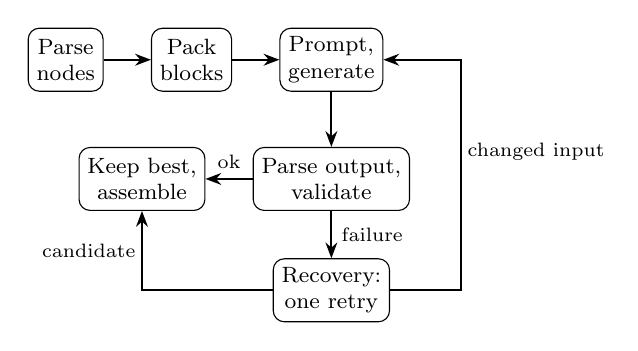
\begin{tikzpicture}[node distance=4mm and 6mm,
  box/.style={draw, rounded corners, align=center, font=\footnotesize, minimum height=8mm, inner sep=3pt},
  arr/.style={-{Stealth[length=2mm]}, thick}]
  \node[box] (parse) {Parse\\nodes};
  \node[box, right=of parse] (pack) {Pack\\blocks};
  \node[box, right=of pack] (gen) {Prompt,\\generate};
  \node[box, below=7mm of gen] (val) {Parse output,\\validate};
  \node[box, left=of val] (sel) {Keep best,\\assemble};
  \node[box, below=6mm of val] (rec) {Recovery:\\one retry};
  \draw[arr] (parse) -- (pack);
  \draw[arr] (pack) -- (gen);
  \draw[arr] (gen) -- (val);
  \draw[arr] (val) -- node[above, font=\scriptsize]{ok} (sel);
  \draw[arr] (val) -- node[right, font=\scriptsize]{failure} (rec);
  \draw[arr] (rec.east) -- ++(9mm,0) |- node[right, pos=0.3, font=\scriptsize, inner sep=2pt]{changed input} (gen.east);
  \draw[arr] (rec.west) -| node[left, pos=0.75, font=\scriptsize, inner sep=2pt]{candidate} (sel.south);
\end{tikzpicture}}
\caption{Document pipeline with one recovery round. At inference the pipeline reads only the source text.}
\label{fig:pipeline}
\end{figure}

Figure~\ref{fig:pipeline} summarises the \texttt{docmt} pipeline, written as one module per step so that each step can be changed and measured alone.

\paragraph{Parse and pack.}
A rule-based parser turns a Markdown document into \emph{nodes} (headings, article and clause labels, paragraphs, table cells, signature blocks) such that concatenating the nodes reproduces the source exactly.
In an earlier version we compared three packings (Section~\ref{sec:results}): one node per request, up to 8 neighbouring nodes (at most 768 source tokens) joined with marker tokens, and the same grouping joined only by newlines.
The submitted version (``legal prose blocks'') first merges adjacent translatable prose nodes of the same scope (headings, articles, clauses, points, list items, paragraphs) into one block, and closes a block once it exceeds 768 source tokens or 8 nodes and its last node ends with a full stop.
A new article or a new chapter or section heading starts a new block, a title chain may join the article that follows it, and tables and signature blocks stay separate units.
Each block is one translation unit and its output is not required to map line by line onto the source nodes, so no line-count check is applied to prose; instead, every source span must be covered exactly once.

\paragraph{Validate and recover.}
Each output is checked for source-span coverage, preserved headings and numbered labels (treating \vi{đ} and \texttt{dd} as the same label), and unfinished generation (no end-of-sequence before the budget, or a detected repetition loop).
A unit with such a failure gets \emph{one} recovery round with a changed input.
After a lost label the prompt adds an instruction to keep the source labels; after a VI$\to$EN unit ran to its budget the earlier (legacy) budget is used; after a repetition loop the repetition penalty is 1.15 \citep{keskar2019ctrl}.
The best translation obtained is kept; a document with unresolved units is still output but flagged, and a span for which the model returns nothing keeps the source text, also flagged, so no content is silently dropped.

\paragraph{Decoding and runtime.}
Decoding is greedy in fp16.
The output budget depends on direction, $\max(256,\lceil 2.5s\rceil{+}128)$ tokens for EN$\to$VI prose and $\max(256,\lceil 1.25s\rceil{+}128)$ for VI$\to$EN prose, where $s$ is the source length; Vietnamese references need about 1.5$\times$ more tokens than English.
Requests are batched by length to reduce padding, and the batch size (8 or 16) is calibrated on each GPU.
In an earlier comparison with the same A1 model, data, budgets and batch size 8, scheduling requests by length cut the public-test wall time of the whole job from 12{,}473 s to 8{,}080 s ($-$35.2\%), with BLEU changing by $-$0.01 (EN$\to$VI) and $+$0.05 (VI$\to$EN).

\paragraph{Anti-repetition.}
A GPU-side detector checks the generated tokens every 32 decoding steps and aborts a degenerate generation early; an aborted unit counts as unfinished and goes to the recovery round above \citep{holtzman2020curious}.
The first pass uses no repetition penalty.
With the same v33 adapter and software environment (single runs), a first-pass penalty of 1.05 scored 70.28 / 47.40 BLEU and 1.0 scored 70.87 / 47.44, so we use no penalty in the first pass; the difference comes from one run per setting and has no confidence interval.
            % Trang  (mục "System" trong dàn ý, đổi tên thành Method)
% Người phụ trách: LINH. (~0,4 trang) -- file giữ chỗ.
% Metric: SacreBLEU 13a (nrefs:1|case:mixed|eff:no|tok:13a|smooth:exp|version:2.6.0), chrF (nc:6|nw:0), bootstrap theo doc (2000 vòng, seed 42).
% Baseline theo dàn ý: model gốc / gốc + pipeline / pipeline + model đã train (Index-2B: Trang_delivery/index_baseline_v33).
\section{Experimental Setup}
\label{sec:setup}
\todo{Linh viết}
             % Linh
% Người phụ trách: LINH. (~1,5 trang) -- file giữ chỗ. Method/Error analysis/Abstract của Trang tham chiếu \ref{sec:results}.
% Số có sẵn (public test, 50 doc x 2 chiều), để Linh đối chiếu với bản mình dùng:
%  - Pipeline A/B/C (A1): EN-VI 68.70/68.90/67.69, VI-EN 46.37/46.62/45.23 ; B-C = +1.21/+1.39 (CI không chứa 0)
%  - FAST16: A1 69.13/46.73 ; v33 70.28/47.40 (rp 1.05) ; delta +1.15 [+0.75,+1.62] / +0.67 [-0.17,+1.79]
%  - Bản nộp (v33, rp 1.0, batch 8, không hậu xử lý): 70.87/47.44 (run/kout/scores.json)
%  - Hậu xử lý xoá chuỗi chấm VI-EN: A1 +1.04, v33 +0.90 (47.40 -> 48.30)
%  - Chi phí: EN-VI 4.54h vs VI-EN 2.87h (B v1.1) ; length batching -21% ; recovery FAST16 840/3739 (EN-VI), 1515/4601 (VI-EN)
%  - Chi phí (nhắc Linh, đề chấm cả thời gian và bộ nhớ): VRAM đỉnh: lấy từ kernel_status.json của run nộp (số 4.55/4.17 GiB người review nêu CHƯA được mình kiểm); EN-VI tốn thời gian hơn vì reference VI dài 1.57x token so với EN
%  - Điểm private 60.4 (README gói FINAL): chưa rõ metric -> hỏi Lâm/Vanh trước khi đưa vào bài
%  - Mọi số v33 trên public test: gắn chú thích '72 dòng term lấy từ reference public (rò nhẹ)'
\section{Results}
\label{sec:results}
\todo{Linh viết}
           % Linh
% Người phụ trách: LINH. (~0,5 trang) -- file giữ chỗ. Theo dàn ý: kết luận ngắn, bỏ Limitations, có thể thêm future work.
\section{Conclusion}
\label{sec:conclusion}
\todo{Linh viết}
        % Linh

\section*{Acknowledgments}
\todo{nhắc người thứ ba làm Hydra (nếu bài có nhắc tới) --- hỏi Linh tên/cách ghi}

\bibliography{refs}

\appendix
% Người phụ trách: TRANG. Đặt SAU References (đã khai báo ở main.tex).
\section{Prompts}
\label{app:prompts}
Both prompts are the ones used in the A1 training script, sent as the user turn of the Hy-MT2 chat template; \texttt{\{src\}} is the unit text and \texttt{\{tgt\}} is ``English'' or ``Vietnamese''.
Inference always uses the default prompt.
\par\vspace{1.4em}
\begin{small}
\noindent\textbf{Default.}\\
\texttt{Translate the following text into \{tgt\}. Note that you should only output the translated result without any additional explanation:\textbackslash n\textbackslash n\{src\}}

\vspace{1.4em}
\noindent\textbf{With terminology (training only).}\\
\texttt{Reference the following translations:\textbackslash n\{refs\}\textbackslash n\textbackslash nTranslate the following text into \{tgt\}. Note that you must ONLY output the translated result without any additional explanation:\textbackslash n\textbackslash n\{src\}}

\smallskip\noindent Each line of \texttt{\{refs\}} is ``\emph{source term} translates to \emph{target term}'', with at most eight pairs.
\end{small}

\section{Hyper-parameters}
\label{app:hyper}
\begin{table}[t]
\centering\small
\begin{tabular}{@{}lp{4.2cm}@{}}
\toprule
\multicolumn{2}{l}{\textit{LoRA fine-tuning (A1, then v33)}}\\
\midrule
Base model & Hy-MT2-1.8B (fixed revision) \\
Adapter & $r{=}64$, $\alpha{=}128$, dropout 0.05 \\
Target modules & q, k, v, o, gate, up, down \\
Trainable parameters & 77.6M (4.15\%) \\
Data & A1: 53.5k pairs; v33: 82{,}203 \\
Learning rate & A1 $2{\times}10^{-4}$; v33 $5{\times}10^{-5}$ \\
Schedule (v33) & cosine to 10\%, 25 warm-up \\
Epochs & 1 (v33: 2{,}569 steps) \\
Batch & $1\times16\times2$ GPUs $=32$ \\
Precision, max length & fp16 DDP, 3{,}072 tokens \\
Weight decay, clip & 0.0, 1.0 \\
Seed, hardware & 42, Kaggle 2$\times$T4 \\
\midrule
\multicolumn{2}{l}{\textit{Inference (submitted setting)}}\\
\midrule
Decoding & greedy, fp16, penalty 1.0 \\
Recovery & one round; penalty 1.15 after a loop \\
Prose block & closed after 768 tokens or 8 nodes, at a full stop \\
Output budget & EN$\to$VI $2.5s{+}128$; VI$\to$EN $1.25s{+}128$ \\
Batch size & 8 (calibrated from 8/16) \\
Context limit & 8{,}192 tokens \\
Post-processing & none \\
\bottomrule
\end{tabular}
\caption{Training and inference settings. $s$ is the source token count; budgets have a floor of 256.}
\label{tab:hyper}
\end{table}

\begingroup\raggedright
\noindent Adapter checksum (SHA-256): {\small\texttt{30b5fc68a31c3de3\allowbreak d722a6dee5484aaf\allowbreak 98c4f6b9d7b41fb5\allowbreak 5ac70f6d23a3ba89}}.\\
\noindent Base model revision: {\small\texttt{9a341cd1b679d3ef\allowbreak d23b46e847b01745\allowbreak a71ed792}}.
\par\endgroup
          % Trang (sau References)

\end{document}
